\documentclass[twoside]{book}

% Packages required by doxygen
\usepackage{calc}
\usepackage{doxygen}
\usepackage{graphicx}
\usepackage[utf8]{inputenc}
\usepackage{makeidx}
\usepackage{multicol}
\usepackage{multirow}
\usepackage{fixltx2e}
\PassOptionsToPackage{warn}{textcomp}
\usepackage{textcomp}
\usepackage[nointegrals]{wasysym}
\usepackage[table]{xcolor}

% Font selection
\usepackage[T1]{fontenc}
\usepackage{mathptmx}
\usepackage[scaled=.90]{helvet}
\usepackage{courier}
\usepackage{amssymb}
\usepackage{sectsty}
\renewcommand{\familydefault}{\sfdefault}
\allsectionsfont{%
  \fontseries{bc}\selectfont%
  \color{darkgray}%
}
\renewcommand{\DoxyLabelFont}{%
  \fontseries{bc}\selectfont%
  \color{darkgray}%
}
\newcommand{\+}{\discretionary{\mbox{\scriptsize$\hookleftarrow$}}{}{}}

% Page & text layout
\usepackage{geometry}
\geometry{%
  a4paper,%
  top=2.5cm,%
  bottom=2.5cm,%
  left=2.5cm,%
  right=2.5cm%
}
\tolerance=750
\hfuzz=15pt
\hbadness=750
\setlength{\emergencystretch}{15pt}
\setlength{\parindent}{0cm}
\setlength{\parskip}{0.2cm}
\makeatletter
\renewcommand{\paragraph}{%
  \@startsection{paragraph}{4}{0ex}{-1.0ex}{1.0ex}{%
    \normalfont\normalsize\bfseries\SS@parafont%
  }%
}
\renewcommand{\subparagraph}{%
  \@startsection{subparagraph}{5}{0ex}{-1.0ex}{1.0ex}{%
    \normalfont\normalsize\bfseries\SS@subparafont%
  }%
}
\makeatother

% Headers & footers
\usepackage{fancyhdr}
\pagestyle{fancyplain}
\fancyhead[LE]{\fancyplain{}{\bfseries\thepage}}
\fancyhead[CE]{\fancyplain{}{}}
\fancyhead[RE]{\fancyplain{}{\bfseries\leftmark}}
\fancyhead[LO]{\fancyplain{}{\bfseries\rightmark}}
\fancyhead[CO]{\fancyplain{}{}}
\fancyhead[RO]{\fancyplain{}{\bfseries\thepage}}
\fancyfoot[LE]{\fancyplain{}{}}
\fancyfoot[CE]{\fancyplain{}{}}
\fancyfoot[RE]{\fancyplain{}{\bfseries\scriptsize Generated on Wed May 21 2014 12\+:52\+:44 for M\+D\+L by Doxygen }}
\fancyfoot[LO]{\fancyplain{}{\bfseries\scriptsize Generated on Wed May 21 2014 12\+:52\+:44 for M\+D\+L by Doxygen }}
\fancyfoot[CO]{\fancyplain{}{}}
\fancyfoot[RO]{\fancyplain{}{}}
\renewcommand{\footrulewidth}{0.4pt}
\renewcommand{\chaptermark}[1]{%
  \markboth{#1}{}%
}
\renewcommand{\sectionmark}[1]{%
  \markright{\thesection\ #1}%
}

% Indices & bibliography
\usepackage{natbib}
\usepackage[titles]{tocloft}
\setcounter{tocdepth}{3}
\setcounter{secnumdepth}{5}
\makeindex

% Hyperlinks (required, but should be loaded last)
\usepackage{ifpdf}
\ifpdf
  \usepackage[pdftex,pagebackref=true]{hyperref}
\else
  \usepackage[ps2pdf,pagebackref=true]{hyperref}
\fi
\hypersetup{%
  colorlinks=true,%
  linkcolor=blue,%
  citecolor=blue,%
  unicode%
}

% Custom commands
\newcommand{\clearemptydoublepage}{%
  \newpage{\pagestyle{empty}\cleardoublepage}%
}


%===== C O N T E N T S =====

\begin{document}

% Titlepage & ToC
\hypersetup{pageanchor=false,
             bookmarks=true,
             bookmarksnumbered=true,
             pdfencoding=unicode
            }
\pagenumbering{roman}
\begin{titlepage}
\vspace*{7cm}
\begin{center}%
{\Large M\+D\+L }\\
\vspace*{1cm}
{\large Generated by Doxygen 1.8.7}\\
\vspace*{0.5cm}
{\small Wed May 21 2014 12:52:44}\\
\end{center}
\end{titlepage}
\clearemptydoublepage
\tableofcontents
\clearemptydoublepage
\pagenumbering{arabic}
\hypersetup{pageanchor=true}

%--- Begin generated contents ---
\chapter{M\+D\+L}
\label{md__r_e_a_d_m_e}
\hypertarget{md__r_e_a_d_m_e}{}
Maison des ligues, application créée dans l'intérêt d'un P\+P\+E pour mon B\+T\+S S\+I\+O option Développeur (S\+L\+A\+M)

A l'aide de \+: Brenda B\+A\+R\+B\+E, Christophe M\+A\+R\+T\+I\+N et Alexandre G\+H\+I\+O. 
\chapter{Namespace Index}
\section{Packages}
Here are the packages with brief descriptions (if available)\+:\begin{DoxyCompactList}
\item\contentsline{section}{\hyperlink{namespace_base_de_donnees}{Base\+De\+Donnees} }{\pageref{namespace_base_de_donnees}}{}
\item\contentsline{section}{\hyperlink{namespace_maison_des_ligues}{Maison\+Des\+Ligues} }{\pageref{namespace_maison_des_ligues}}{}
\item\contentsline{section}{\hyperlink{namespace_maison_des_ligues_1_1_properties}{Maison\+Des\+Ligues.\+Properties} }{\pageref{namespace_maison_des_ligues_1_1_properties}}{}
\end{DoxyCompactList}

\chapter{Hierarchical Index}
\section{Class Hierarchy}
This inheritance list is sorted roughly, but not completely, alphabetically\+:\begin{DoxyCompactList}
\item \contentsline{section}{Base\+De\+Donnees.\+Bdd}{\pageref{class_base_de_donnees_1_1_bdd}}{}
\item Form\begin{DoxyCompactList}
\item \contentsline{section}{Maison\+Des\+Ligues.\+Form\+Ajout\+Atelier}{\pageref{class_maison_des_ligues_1_1_form_ajout_atelier}}{}
\item \contentsline{section}{Maison\+Des\+Ligues.\+Form\+Ajout\+Theme}{\pageref{class_maison_des_ligues_1_1_form_ajout_theme}}{}
\item \contentsline{section}{Maison\+Des\+Ligues.\+Form\+Ajout\+Vacation}{\pageref{class_maison_des_ligues_1_1_form_ajout_vacation}}{}
\item \contentsline{section}{Maison\+Des\+Ligues.\+Form\+Modifi\+Vacation}{\pageref{class_maison_des_ligues_1_1_form_modifi_vacation}}{}
\item \contentsline{section}{Maison\+Des\+Ligues.\+Frm\+Login}{\pageref{class_maison_des_ligues_1_1_frm_login}}{}
\item \contentsline{section}{Maison\+Des\+Ligues.\+Frm\+Principale}{\pageref{class_maison_des_ligues_1_1_frm_principale}}{}
\end{DoxyCompactList}
\end{DoxyCompactList}

\chapter{Class Index}
\section{Class List}
Here are the classes, structs, unions and interfaces with brief descriptions\+:\begin{DoxyCompactList}
\item\contentsline{section}{\hyperlink{class_base_de_donnees_1_1_bdd}{Base\+De\+Donnees.\+Bdd} }{\pageref{class_base_de_donnees_1_1_bdd}}{}
\item\contentsline{section}{\hyperlink{class_maison_des_ligues_1_1_form_ajout_atelier}{Maison\+Des\+Ligues.\+Form\+Ajout\+Atelier} }{\pageref{class_maison_des_ligues_1_1_form_ajout_atelier}}{}
\item\contentsline{section}{\hyperlink{class_maison_des_ligues_1_1_form_ajout_theme}{Maison\+Des\+Ligues.\+Form\+Ajout\+Theme} }{\pageref{class_maison_des_ligues_1_1_form_ajout_theme}}{}
\item\contentsline{section}{\hyperlink{class_maison_des_ligues_1_1_form_ajout_vacation}{Maison\+Des\+Ligues.\+Form\+Ajout\+Vacation} }{\pageref{class_maison_des_ligues_1_1_form_ajout_vacation}}{}
\item\contentsline{section}{\hyperlink{class_maison_des_ligues_1_1_form_modifi_vacation}{Maison\+Des\+Ligues.\+Form\+Modifi\+Vacation} }{\pageref{class_maison_des_ligues_1_1_form_modifi_vacation}}{}
\item\contentsline{section}{\hyperlink{class_maison_des_ligues_1_1_frm_login}{Maison\+Des\+Ligues.\+Frm\+Login} }{\pageref{class_maison_des_ligues_1_1_frm_login}}{}
\item\contentsline{section}{\hyperlink{class_maison_des_ligues_1_1_frm_principale}{Maison\+Des\+Ligues.\+Frm\+Principale} }{\pageref{class_maison_des_ligues_1_1_frm_principale}}{}
\end{DoxyCompactList}

\chapter{Namespace Documentation}
\hypertarget{namespace_base_de_donnees}{\section{Package Base\+De\+Donnees}
\label{namespace_base_de_donnees}\index{Base\+De\+Donnees@{Base\+De\+Donnees}}
}
\subsection*{Classes}
\begin{DoxyCompactItemize}
\item 
class \hyperlink{class_base_de_donnees_1_1_bdd}{Bdd}
\end{DoxyCompactItemize}

\hypertarget{namespace_maison_des_ligues}{\section{Package Maison\+Des\+Ligues}
\label{namespace_maison_des_ligues}\index{Maison\+Des\+Ligues@{Maison\+Des\+Ligues}}
}
\subsection*{Namespaces}
\begin{DoxyCompactItemize}
\item 
package \hyperlink{namespace_maison_des_ligues_1_1_properties}{Properties}
\end{DoxyCompactItemize}
\subsection*{Classes}
\begin{DoxyCompactItemize}
\item 
class \hyperlink{class_maison_des_ligues_1_1_form_ajout_atelier}{Form\+Ajout\+Atelier}
\item 
class \hyperlink{class_maison_des_ligues_1_1_form_ajout_theme}{Form\+Ajout\+Theme}
\item 
class \hyperlink{class_maison_des_ligues_1_1_form_ajout_vacation}{Form\+Ajout\+Vacation}
\item 
class \hyperlink{class_maison_des_ligues_1_1_form_modifi_vacation}{Form\+Modifi\+Vacation}
\item 
class \hyperlink{class_maison_des_ligues_1_1_frm_login}{Frm\+Login}
\item 
class \hyperlink{class_maison_des_ligues_1_1_frm_principale}{Frm\+Principale}
\item 
class {\bfseries Program}
\item 
class {\bfseries Utilitaire}
\end{DoxyCompactItemize}

\hypertarget{namespace_maison_des_ligues_1_1_properties}{\section{Package Maison\+Des\+Ligues.\+Properties}
\label{namespace_maison_des_ligues_1_1_properties}\index{Maison\+Des\+Ligues.\+Properties@{Maison\+Des\+Ligues.\+Properties}}
}
\subsection*{Classes}
\begin{DoxyCompactItemize}
\item 
class {\bfseries Resources}
\begin{DoxyCompactList}\small\item\em Une classe de ressource fortement typée destinée, entre autres, à la consultation des chaînes localisées. \end{DoxyCompactList}\item 
class {\bfseries Settings}
\end{DoxyCompactItemize}

\chapter{Class Documentation}
\hypertarget{class_base_de_donnees_1_1_bdd}{\section{Base\+De\+Donnees.\+Bdd Class Reference}
\label{class_base_de_donnees_1_1_bdd}\index{Base\+De\+Donnees.\+Bdd@{Base\+De\+Donnees.\+Bdd}}
}
\subsection*{Public Member Functions}
\begin{DoxyCompactItemize}
\item 
\hyperlink{class_base_de_donnees_1_1_bdd_ab7425636f7b6865411160424455ddacf}{Bdd} (String Un\+Login, String Un\+Pwd)
\begin{DoxyCompactList}\small\item\em constructeur de la connexion \end{DoxyCompactList}\item 
void \hyperlink{class_base_de_donnees_1_1_bdd_aa75a70827f654db3f17b9451975446bb}{Fermer\+Connexion} ()
\begin{DoxyCompactList}\small\item\em Méthode permettant de fermer la connexion \end{DoxyCompactList}\item 
Data\+Table \hyperlink{class_base_de_donnees_1_1_bdd_a1f5203fd6378328a9545b47b7dd6bd97}{Obtenir\+Donnes\+Oracle} (String Une\+Table\+Ou\+Vue)
\begin{DoxyCompactList}\small\item\em permet de récupérer le contenu d'une table ou d'une vue. \end{DoxyCompactList}\item 
void \hyperlink{class_base_de_donnees_1_1_bdd_ac60e11f0e915babf2a78d168bf7a744e}{Inscrire\+Benevole} (String p\+Nom, String p\+Prenom, String p\+Adresse1, String p\+Adresse2, String p\+Cp, String p\+Ville, String p\+Tel, String p\+Mail, Date\+Time p\+Date\+Naissance, Int64?p\+Numero\+Licence, Collection$<$ Int16 $>$ p\+Date\+Benevolat)
\begin{DoxyCompactList}\small\item\em procédure qui va se charger d'invoquer la procédure stockée qui ira inscrire un participant de type bénévole \end{DoxyCompactList}\item 
void \hyperlink{class_base_de_donnees_1_1_bdd_abfbf2eb771a5e60ef361d5d9fc00304f}{Inscrire\+Intervenant} (String p\+Nom, String p\+Prenom, String p\+Adresse1, String p\+Adresse2, String p\+Cp, String p\+Ville, String p\+Tel, String p\+Mail, Int16 p\+Id\+Atelier, String p\+Id\+Statut)
\begin{DoxyCompactList}\small\item\em Procédure publique qui va appeler la procédure stockée permettant d'inscrire un nouvel intervenant sans nuité \end{DoxyCompactList}\item 
void \hyperlink{class_base_de_donnees_1_1_bdd_a2ecae01b408afab3f2457286b9bc6cc7}{Inscrire\+Intervenant} (String p\+Nom, String p\+Prenom, String p\+Adresse1, String p\+Adresse2, String p\+Cp, String p\+Ville, String p\+Tel, String p\+Mail, Int16 p\+Id\+Atelier, String p\+Id\+Statut, Collection$<$ string $>$ p\+Les\+Categories, Collection$<$ string $>$ p\+Les\+Hotels, Collection$<$ Int16 $>$ p\+Les\+Nuits)
\begin{DoxyCompactList}\small\item\em Procédure publique qui va appeler la procédure stockée permettant d'inscrire un nouvel intervenant qui aura des nuités \end{DoxyCompactList}\item 
Dictionary$<$ Int16, String $>$ \hyperlink{class_base_de_donnees_1_1_bdd_af48b871d33fdfd845de9d4012109d00f}{Obtenir\+Dates\+Nuites} ()
\begin{DoxyCompactList}\small\item\em fonction permettant de construire un dictionnaire dont l'id est l'id d'une nuité et le contenu une date sous la la forme \+: lundi 7 janvier 2013 /// \end{DoxyCompactList}\item 
\hypertarget{class_base_de_donnees_1_1_bdd_a8d465aeda4c9f18878abfdd9c73458d7}{Dictionary$<$ Int16, String $>$ {\bfseries Obtenir\+Atelier} ()}\label{class_base_de_donnees_1_1_bdd_a8d465aeda4c9f18878abfdd9c73458d7}

\item 
void \hyperlink{class_base_de_donnees_1_1_bdd_a47e6453dc9e7851ca41b8d68a358214f}{Inscrire\+Licencie} (String p\+Nom, String p\+Prenom, String p\+Adresse1, String p\+Adresse2, String p\+Cp, String p\+Ville, String p\+Tel, String p\+Mail, Int16 p\+Id\+Qualite, Int64 p\+Numero\+Licence, Collection$<$ Int16 $>$ p\+Les\+Ateliers, Int64 p\+Num\+Cheque, Double p\+Montant\+Cheque, Collection$<$ Int16 $>$ p\+Les\+Accompagnants, String p\+Inscription)
\begin{DoxyCompactList}\small\item\em Procédure publique qui va appeler la procédure stockée permettant d'inscrire un nouvel licencié avec nuité \end{DoxyCompactList}\item 
void \hyperlink{class_base_de_donnees_1_1_bdd_aeea37a4bfb9bf95ef02f350c39d003f4}{Inscrire\+Licencie} (String p\+Nom, String p\+Prenom, String p\+Adresse1, String p\+Adresse2, String p\+Cp, String p\+Ville, String p\+Tel, String p\+Mail, Int16 p\+Id\+Qualite, Int64 p\+Numero\+Licence, Collection$<$ Int16 $>$ p\+Les\+Ateliers, Collection$<$ string $>$ p\+Les\+Categories, Collection$<$ string $>$ p\+Les\+Hotels, Collection$<$ Int16 $>$ p\+Les\+Nuits, Int64 p\+Num\+Cheque, Double p\+Montant\+Cheque, Collection$<$ Int16 $>$ p\+Les\+Accompagnants, String p\+Inscription)
\begin{DoxyCompactList}\small\item\em Procédure publique qui va appeler la procédure stockée permettant d'inscrire un nouvel intervenant sans nuité \end{DoxyCompactList}\item 
void \hyperlink{class_base_de_donnees_1_1_bdd_a32cef1502d8342b040476519c7b6df1e}{Enregistrer\+Paiement} (Double p\+Montant\+Cheque, Int64 p\+Numero\+Cheque, Int64 p\+Numero\+Licencie, String p\+Type\+Paiement)
\begin{DoxyCompactList}\small\item\em Fonction qui permet d'enregistrer un paiement \end{DoxyCompactList}\item 
void \hyperlink{class_base_de_donnees_1_1_bdd_a5c46dd24715a9f9c7298f965963f632c}{ajout\+Atelier} (string Libelle, int Nb\+Places\+Maxi)
\begin{DoxyCompactList}\small\item\em Fonction permettant d'ajouter un nouvel atelier \end{DoxyCompactList}\item 
void \hyperlink{class_base_de_donnees_1_1_bdd_a01351c579bdfe073813f741ce33e54ce}{ajout\+Theme} (int id\+Atelier, int numero, string libelle\+Theme)
\begin{DoxyCompactList}\small\item\em Fonction permettant d'ajouter un theme \end{DoxyCompactList}\item 
void \hyperlink{class_base_de_donnees_1_1_bdd_ad7aa89a1bbf10e7a5996fb93634d72fe}{ajout\+Vacation} (int id\+Atelier, int numero, string date\+Heure\+Debut, string date\+Heurefin)
\begin{DoxyCompactList}\small\item\em Fonction permettant d'ajouter une vacation \end{DoxyCompactList}\item 
void \hyperlink{class_base_de_donnees_1_1_bdd_a7c2205af82b45cce1c03a2dd9bc00aa9}{modif\+Vacation} (int id\+Atelier, int numero, string date\+Heure\+Debut, string date\+Heure\+Fin)
\begin{DoxyCompactList}\small\item\em Fonction permettant de modifier les dates et heures d'une vacation \end{DoxyCompactList}\item 
Data\+Table \hyperlink{class_base_de_donnees_1_1_bdd_ab255932540cdc034e41a6d526e3e5c62}{Obtenir\+Id\+Atelier\+Vacation} ()
\begin{DoxyCompactList}\small\item\em Fonction qui retourne tout les ateliers qui sont en relations avec des vacations \end{DoxyCompactList}\end{DoxyCompactItemize}


\subsection{Constructor \& Destructor Documentation}
\hypertarget{class_base_de_donnees_1_1_bdd_ab7425636f7b6865411160424455ddacf}{\index{Base\+De\+Donnees\+::\+Bdd@{Base\+De\+Donnees\+::\+Bdd}!Bdd@{Bdd}}
\index{Bdd@{Bdd}!Base\+De\+Donnees\+::\+Bdd@{Base\+De\+Donnees\+::\+Bdd}}
\subsubsection[{Bdd}]{\setlength{\rightskip}{0pt plus 5cm}Base\+De\+Donnees.\+Bdd.\+Bdd (
\begin{DoxyParamCaption}
\item[{String}]{Un\+Login, }
\item[{String}]{Un\+Pwd}
\end{DoxyParamCaption}
)}}\label{class_base_de_donnees_1_1_bdd_ab7425636f7b6865411160424455ddacf}


constructeur de la connexion 


\begin{DoxyParams}{Parameters}
{\em Un\+Login} & login utilisateur\\
\hline
{\em Un\+Pwd} & mot de passe utilisateur\\
\hline
\end{DoxyParams}
on commence par récupérer dans Cn\+String les informations contenues dans le fichier app.\+config pour la connection\+String de nom Str\+Conn\+Mdl 

on va remplacer dans la chaine de connexion les paramètres par le login et le pwd saisis dans les zones de texte. Pour ça on va utiliser la méthode Format de la classe String. /// 

\subsection{Member Function Documentation}
\hypertarget{class_base_de_donnees_1_1_bdd_a5c46dd24715a9f9c7298f965963f632c}{\index{Base\+De\+Donnees\+::\+Bdd@{Base\+De\+Donnees\+::\+Bdd}!ajout\+Atelier@{ajout\+Atelier}}
\index{ajout\+Atelier@{ajout\+Atelier}!Base\+De\+Donnees\+::\+Bdd@{Base\+De\+Donnees\+::\+Bdd}}
\subsubsection[{ajout\+Atelier}]{\setlength{\rightskip}{0pt plus 5cm}void Base\+De\+Donnees.\+Bdd.\+ajout\+Atelier (
\begin{DoxyParamCaption}
\item[{string}]{Libelle, }
\item[{int}]{Nb\+Places\+Maxi}
\end{DoxyParamCaption}
)}}\label{class_base_de_donnees_1_1_bdd_a5c46dd24715a9f9c7298f965963f632c}


Fonction permettant d'ajouter un nouvel atelier 


\begin{DoxyParams}{Parameters}
{\em Libelle} & Libelle de l'atelier\\
\hline
{\em Nb\+Places\+Maxi} & Nombre de places que peut accueillir l'atelier\\
\hline
\end{DoxyParams}
\hypertarget{class_base_de_donnees_1_1_bdd_a01351c579bdfe073813f741ce33e54ce}{\index{Base\+De\+Donnees\+::\+Bdd@{Base\+De\+Donnees\+::\+Bdd}!ajout\+Theme@{ajout\+Theme}}
\index{ajout\+Theme@{ajout\+Theme}!Base\+De\+Donnees\+::\+Bdd@{Base\+De\+Donnees\+::\+Bdd}}
\subsubsection[{ajout\+Theme}]{\setlength{\rightskip}{0pt plus 5cm}void Base\+De\+Donnees.\+Bdd.\+ajout\+Theme (
\begin{DoxyParamCaption}
\item[{int}]{id\+Atelier, }
\item[{int}]{numero, }
\item[{string}]{libelle\+Theme}
\end{DoxyParamCaption}
)}}\label{class_base_de_donnees_1_1_bdd_a01351c579bdfe073813f741ce33e54ce}


Fonction permettant d'ajouter un theme 


\begin{DoxyParams}{Parameters}
{\em id\+Atelier} & Id de l'atelier concerné par le nouveau theme\\
\hline
{\em numero} & Numéro du thème\\
\hline
{\em libelle\+Theme} & Libelle du thème\\
\hline
\end{DoxyParams}
\hypertarget{class_base_de_donnees_1_1_bdd_ad7aa89a1bbf10e7a5996fb93634d72fe}{\index{Base\+De\+Donnees\+::\+Bdd@{Base\+De\+Donnees\+::\+Bdd}!ajout\+Vacation@{ajout\+Vacation}}
\index{ajout\+Vacation@{ajout\+Vacation}!Base\+De\+Donnees\+::\+Bdd@{Base\+De\+Donnees\+::\+Bdd}}
\subsubsection[{ajout\+Vacation}]{\setlength{\rightskip}{0pt plus 5cm}void Base\+De\+Donnees.\+Bdd.\+ajout\+Vacation (
\begin{DoxyParamCaption}
\item[{int}]{id\+Atelier, }
\item[{int}]{numero, }
\item[{string}]{date\+Heure\+Debut, }
\item[{string}]{date\+Heurefin}
\end{DoxyParamCaption}
)}}\label{class_base_de_donnees_1_1_bdd_ad7aa89a1bbf10e7a5996fb93634d72fe}


Fonction permettant d'ajouter une vacation 


\begin{DoxyParams}{Parameters}
{\em id\+Atelier} & Id de l'atelier concernée\\
\hline
{\em numero} & numero\\
\hline
{\em date\+Heure\+Debut} & Date et heure de début de la vacation\\
\hline
{\em date\+Heurefin} & Date et heure de fin de la vacation\\
\hline
\end{DoxyParams}
\hypertarget{class_base_de_donnees_1_1_bdd_a32cef1502d8342b040476519c7b6df1e}{\index{Base\+De\+Donnees\+::\+Bdd@{Base\+De\+Donnees\+::\+Bdd}!Enregistrer\+Paiement@{Enregistrer\+Paiement}}
\index{Enregistrer\+Paiement@{Enregistrer\+Paiement}!Base\+De\+Donnees\+::\+Bdd@{Base\+De\+Donnees\+::\+Bdd}}
\subsubsection[{Enregistrer\+Paiement}]{\setlength{\rightskip}{0pt plus 5cm}void Base\+De\+Donnees.\+Bdd.\+Enregistrer\+Paiement (
\begin{DoxyParamCaption}
\item[{Double}]{p\+Montant\+Cheque, }
\item[{Int64}]{p\+Numero\+Cheque, }
\item[{Int64}]{p\+Numero\+Licencie, }
\item[{String}]{p\+Type\+Paiement}
\end{DoxyParamCaption}
)}}\label{class_base_de_donnees_1_1_bdd_a32cef1502d8342b040476519c7b6df1e}


Fonction qui permet d'enregistrer un paiement 


\begin{DoxyParams}{Parameters}
{\em p\+Montant\+Cheque} & Numero du cheque du licencie\\
\hline
{\em p\+Numero\+Cheque} & Numero du cheque du licencie\\
\hline
{\em p\+Numero\+Licencie} & Numero de licence du licencie\\
\hline
{\em p\+Type\+Paiement} & Type de paiement du licencie\\
\hline
\end{DoxyParams}
\hypertarget{class_base_de_donnees_1_1_bdd_aa75a70827f654db3f17b9451975446bb}{\index{Base\+De\+Donnees\+::\+Bdd@{Base\+De\+Donnees\+::\+Bdd}!Fermer\+Connexion@{Fermer\+Connexion}}
\index{Fermer\+Connexion@{Fermer\+Connexion}!Base\+De\+Donnees\+::\+Bdd@{Base\+De\+Donnees\+::\+Bdd}}
\subsubsection[{Fermer\+Connexion}]{\setlength{\rightskip}{0pt plus 5cm}void Base\+De\+Donnees.\+Bdd.\+Fermer\+Connexion (
\begin{DoxyParamCaption}
{}
\end{DoxyParamCaption}
)}}\label{class_base_de_donnees_1_1_bdd_aa75a70827f654db3f17b9451975446bb}


Méthode permettant de fermer la connexion 

\hypertarget{class_base_de_donnees_1_1_bdd_ac60e11f0e915babf2a78d168bf7a744e}{\index{Base\+De\+Donnees\+::\+Bdd@{Base\+De\+Donnees\+::\+Bdd}!Inscrire\+Benevole@{Inscrire\+Benevole}}
\index{Inscrire\+Benevole@{Inscrire\+Benevole}!Base\+De\+Donnees\+::\+Bdd@{Base\+De\+Donnees\+::\+Bdd}}
\subsubsection[{Inscrire\+Benevole}]{\setlength{\rightskip}{0pt plus 5cm}void Base\+De\+Donnees.\+Bdd.\+Inscrire\+Benevole (
\begin{DoxyParamCaption}
\item[{String}]{p\+Nom, }
\item[{String}]{p\+Prenom, }
\item[{String}]{p\+Adresse1, }
\item[{String}]{p\+Adresse2, }
\item[{String}]{p\+Cp, }
\item[{String}]{p\+Ville, }
\item[{String}]{p\+Tel, }
\item[{String}]{p\+Mail, }
\item[{Date\+Time}]{p\+Date\+Naissance, }
\item[{Int64?}]{p\+Numero\+Licence, }
\item[{Collection$<$ Int16 $>$}]{p\+Date\+Benevolat}
\end{DoxyParamCaption}
)}}\label{class_base_de_donnees_1_1_bdd_ac60e11f0e915babf2a78d168bf7a744e}


procédure qui va se charger d'invoquer la procédure stockée qui ira inscrire un participant de type bénévole 


\begin{DoxyParams}{Parameters}
{\em Cmd} & nom de l'objet command concerné par les paramètres\\
\hline
{\em p\+Nom} & nom du participant\\
\hline
{\em p\+Prenom} & prénom du participant\\
\hline
{\em p\+Adresse1} & adresse1 du participant\\
\hline
{\em p\+Adresse2} & adresse2 du participant\\
\hline
{\em p\+Cp} & cp du participant\\
\hline
{\em p\+Ville} & ville du participant\\
\hline
{\em p\+Tel} & téléphone du participant\\
\hline
{\em p\+Mail} & mail du participant\\
\hline
{\em p\+Date\+Naissance} & mail du bénévole\\
\hline
{\em p\+Numero\+Licence} & numéro de licence du bénévole ou null\\
\hline
{\em p\+Date\+Benevolat} & collection des id des dates où le bénévole sera présent\\
\hline
\end{DoxyParams}
\hypertarget{class_base_de_donnees_1_1_bdd_abfbf2eb771a5e60ef361d5d9fc00304f}{\index{Base\+De\+Donnees\+::\+Bdd@{Base\+De\+Donnees\+::\+Bdd}!Inscrire\+Intervenant@{Inscrire\+Intervenant}}
\index{Inscrire\+Intervenant@{Inscrire\+Intervenant}!Base\+De\+Donnees\+::\+Bdd@{Base\+De\+Donnees\+::\+Bdd}}
\subsubsection[{Inscrire\+Intervenant}]{\setlength{\rightskip}{0pt plus 5cm}void Base\+De\+Donnees.\+Bdd.\+Inscrire\+Intervenant (
\begin{DoxyParamCaption}
\item[{String}]{p\+Nom, }
\item[{String}]{p\+Prenom, }
\item[{String}]{p\+Adresse1, }
\item[{String}]{p\+Adresse2, }
\item[{String}]{p\+Cp, }
\item[{String}]{p\+Ville, }
\item[{String}]{p\+Tel, }
\item[{String}]{p\+Mail, }
\item[{Int16}]{p\+Id\+Atelier, }
\item[{String}]{p\+Id\+Statut}
\end{DoxyParamCaption}
)}}\label{class_base_de_donnees_1_1_bdd_abfbf2eb771a5e60ef361d5d9fc00304f}


Procédure publique qui va appeler la procédure stockée permettant d'inscrire un nouvel intervenant sans nuité 


\begin{DoxyParams}{Parameters}
{\em Cmd} & nom de l'objet command concerné par les paramètres\\
\hline
{\em p\+Nom} & nom du participant\\
\hline
{\em p\+Prenom} & prénom du participant\\
\hline
{\em p\+Adresse1} & adresse1 du participant\\
\hline
{\em p\+Adresse2} & adresse2 du participant\\
\hline
{\em p\+Cp} & cp du participant\\
\hline
{\em p\+Ville} & ville du participant\\
\hline
{\em p\+Tel} & téléphone du participant\\
\hline
{\em p\+Mail} & mail du participant\\
\hline
{\em p\+Id\+Atelier} & Id de l'atelier où interviendra l'intervenant\\
\hline
{\em p\+Id\+Statut} & statut de l'intervenant pour l'atelier \+: animateur ou intervenant\\
\hline
\end{DoxyParams}
procédure qui va créer \+: 1-\/ un enregistrement dans la table participant 2-\/ un enregistrement dans la table intervenant en cas d'erreur Oracle, appel à la méthode Get\+Message\+Oracle dont le rôle est d'extraire uniquement le message renvoyé par une procédure ou un trigger Oracle \hypertarget{class_base_de_donnees_1_1_bdd_a2ecae01b408afab3f2457286b9bc6cc7}{\index{Base\+De\+Donnees\+::\+Bdd@{Base\+De\+Donnees\+::\+Bdd}!Inscrire\+Intervenant@{Inscrire\+Intervenant}}
\index{Inscrire\+Intervenant@{Inscrire\+Intervenant}!Base\+De\+Donnees\+::\+Bdd@{Base\+De\+Donnees\+::\+Bdd}}
\subsubsection[{Inscrire\+Intervenant}]{\setlength{\rightskip}{0pt plus 5cm}void Base\+De\+Donnees.\+Bdd.\+Inscrire\+Intervenant (
\begin{DoxyParamCaption}
\item[{String}]{p\+Nom, }
\item[{String}]{p\+Prenom, }
\item[{String}]{p\+Adresse1, }
\item[{String}]{p\+Adresse2, }
\item[{String}]{p\+Cp, }
\item[{String}]{p\+Ville, }
\item[{String}]{p\+Tel, }
\item[{String}]{p\+Mail, }
\item[{Int16}]{p\+Id\+Atelier, }
\item[{String}]{p\+Id\+Statut, }
\item[{Collection$<$ string $>$}]{p\+Les\+Categories, }
\item[{Collection$<$ string $>$}]{p\+Les\+Hotels, }
\item[{Collection$<$ Int16 $>$}]{p\+Les\+Nuits}
\end{DoxyParamCaption}
)}}\label{class_base_de_donnees_1_1_bdd_a2ecae01b408afab3f2457286b9bc6cc7}


Procédure publique qui va appeler la procédure stockée permettant d'inscrire un nouvel intervenant qui aura des nuités 


\begin{DoxyParams}{Parameters}
{\em Cmd} & nom de l'objet command concerné par les paramètres\\
\hline
{\em p\+Nom} & nom du participant\\
\hline
{\em p\+Prenom} & prénom du participant\\
\hline
{\em p\+Adresse1} & adresse1 du participant\\
\hline
{\em p\+Adresse2} & adresse2 du participant\\
\hline
{\em p\+Cp} & cp du participant\\
\hline
{\em p\+Ville} & ville du participant\\
\hline
{\em p\+Tel} & téléphone du participant\\
\hline
{\em p\+Mail} & mail du participant\\
\hline
{\em p\+Id\+Atelier} & Id de l'atelier où interviendra l'intervenant\\
\hline
{\em p\+Id\+Statut} & statut de l'intervenant pour l'atelier \+: animateur ou intervenant\\
\hline
{\em p\+Les\+Categories} & tableau contenant la catégorie de chambre pour chaque nuité à réserver\\
\hline
{\em p\+Les\+Hotels} & tableau contenant l'hôtel pour chaque nuité à réserver\\
\hline
{\em p\+Les\+Nuits} & tableau contenant l'id de la date d'arrivée pour chaque nuité à réserver\\
\hline
\end{DoxyParams}
procédure qui va \+: 1-\/ faire appel à la procédure un enregistrement dans la table participant 2-\/ un enregistrement dans la table intervenant 3-\/ un à 2 enregistrements dans la table C\+O\+N\+T\+E\+N\+U\+H\+E\+B\+E\+R\+G\+E\+M\+E\+N\+T

en cas d'erreur Oracle, appel à la méthode Get\+Message\+Oracle dont le rôle est d'extraire uniquement le message renvoyé par une procédure ou un trigger Oracle \hypertarget{class_base_de_donnees_1_1_bdd_a47e6453dc9e7851ca41b8d68a358214f}{\index{Base\+De\+Donnees\+::\+Bdd@{Base\+De\+Donnees\+::\+Bdd}!Inscrire\+Licencie@{Inscrire\+Licencie}}
\index{Inscrire\+Licencie@{Inscrire\+Licencie}!Base\+De\+Donnees\+::\+Bdd@{Base\+De\+Donnees\+::\+Bdd}}
\subsubsection[{Inscrire\+Licencie}]{\setlength{\rightskip}{0pt plus 5cm}void Base\+De\+Donnees.\+Bdd.\+Inscrire\+Licencie (
\begin{DoxyParamCaption}
\item[{String}]{p\+Nom, }
\item[{String}]{p\+Prenom, }
\item[{String}]{p\+Adresse1, }
\item[{String}]{p\+Adresse2, }
\item[{String}]{p\+Cp, }
\item[{String}]{p\+Ville, }
\item[{String}]{p\+Tel, }
\item[{String}]{p\+Mail, }
\item[{Int16}]{p\+Id\+Qualite, }
\item[{Int64}]{p\+Numero\+Licence, }
\item[{Collection$<$ Int16 $>$}]{p\+Les\+Ateliers, }
\item[{Int64}]{p\+Num\+Cheque, }
\item[{Double}]{p\+Montant\+Cheque, }
\item[{Collection$<$ Int16 $>$}]{p\+Les\+Accompagnants, }
\item[{String}]{p\+Inscription}
\end{DoxyParamCaption}
)}}\label{class_base_de_donnees_1_1_bdd_a47e6453dc9e7851ca41b8d68a358214f}


Procédure publique qui va appeler la procédure stockée permettant d'inscrire un nouvel licencié avec nuité 


\begin{DoxyParams}{Parameters}
{\em Cmd} & nom de l'objet command concerné par les paramètres\\
\hline
{\em p\+Nom} & nom du participant\\
\hline
{\em p\+Prenom} & prénom du participant\\
\hline
{\em p\+Adresse1} & adresse1 du participant\\
\hline
{\em p\+Adresse2} & adresse2 du participant\\
\hline
{\em p\+Cp} & cp du participant\\
\hline
{\em p\+Ville} & ville du participant\\
\hline
{\em p\+Tel} & téléphone du participant\\
\hline
{\em p\+Mail} & mail du participant\\
\hline
{\em p\+Id\+Qualite} & qualité du licencié\\
\hline
{\em p\+Numero\+Licence} & numéro de licence du licencié\\
\hline
{\em p\+Les\+Ateliers} & collection des ateliers du licencié\\
\hline
{\em p\+Num\+Cheque} & numéro de cheque du licencié\\
\hline
{\em p\+Montant\+Cheque} & montant du cheque du licencié\\
\hline
{\em p\+Les\+Accompagnants} & collection des accompagnants du licencié\\
\hline
{\em p\+Inscription} & type du paiement du licencié\\
\hline
\end{DoxyParams}
\hypertarget{class_base_de_donnees_1_1_bdd_aeea37a4bfb9bf95ef02f350c39d003f4}{\index{Base\+De\+Donnees\+::\+Bdd@{Base\+De\+Donnees\+::\+Bdd}!Inscrire\+Licencie@{Inscrire\+Licencie}}
\index{Inscrire\+Licencie@{Inscrire\+Licencie}!Base\+De\+Donnees\+::\+Bdd@{Base\+De\+Donnees\+::\+Bdd}}
\subsubsection[{Inscrire\+Licencie}]{\setlength{\rightskip}{0pt plus 5cm}void Base\+De\+Donnees.\+Bdd.\+Inscrire\+Licencie (
\begin{DoxyParamCaption}
\item[{String}]{p\+Nom, }
\item[{String}]{p\+Prenom, }
\item[{String}]{p\+Adresse1, }
\item[{String}]{p\+Adresse2, }
\item[{String}]{p\+Cp, }
\item[{String}]{p\+Ville, }
\item[{String}]{p\+Tel, }
\item[{String}]{p\+Mail, }
\item[{Int16}]{p\+Id\+Qualite, }
\item[{Int64}]{p\+Numero\+Licence, }
\item[{Collection$<$ Int16 $>$}]{p\+Les\+Ateliers, }
\item[{Collection$<$ string $>$}]{p\+Les\+Categories, }
\item[{Collection$<$ string $>$}]{p\+Les\+Hotels, }
\item[{Collection$<$ Int16 $>$}]{p\+Les\+Nuits, }
\item[{Int64}]{p\+Num\+Cheque, }
\item[{Double}]{p\+Montant\+Cheque, }
\item[{Collection$<$ Int16 $>$}]{p\+Les\+Accompagnants, }
\item[{String}]{p\+Inscription}
\end{DoxyParamCaption}
)}}\label{class_base_de_donnees_1_1_bdd_aeea37a4bfb9bf95ef02f350c39d003f4}


Procédure publique qui va appeler la procédure stockée permettant d'inscrire un nouvel intervenant sans nuité 


\begin{DoxyParams}{Parameters}
{\em Cmd} & nom de l'objet command concerné par les paramètres\\
\hline
{\em p\+Nom} & nom du participant\\
\hline
{\em p\+Prenom} & prénom du participant\\
\hline
{\em p\+Adresse1} & adresse1 du participant\\
\hline
{\em p\+Adresse2} & adresse2 du participant\\
\hline
{\em p\+Cp} & cp du participant\\
\hline
{\em p\+Ville} & ville du participant\\
\hline
{\em p\+Tel} & téléphone du participant\\
\hline
{\em p\+Mail} & mail du participant\\
\hline
{\em p\+Id\+Qualite} & qualité du licencié\\
\hline
{\em p\+Numero\+Licence} & numéro de licence du licencié\\
\hline
{\em p\+Les\+Ateliers} & collection des ateliers du licencié\\
\hline
{\em p\+Les\+Categories} & collection des catégories de l'hotel du licencié\\
\hline
{\em p\+Les\+Hotels} & collection des hotels du licencié\\
\hline
{\em p\+Les\+Nuits} & collection des nuits du licencié\\
\hline
{\em p\+Num\+Cheque} & numéro du cheque du licencié\\
\hline
{\em p\+Montant\+Cheque} & montant du cheque du licencié\\
\hline
{\em p\+Les\+Accompagnants} & collection des accompagnants du licencié\\
\hline
{\em p\+Inscription} & type du paiement du licencié\\
\hline
\end{DoxyParams}
\hypertarget{class_base_de_donnees_1_1_bdd_a7c2205af82b45cce1c03a2dd9bc00aa9}{\index{Base\+De\+Donnees\+::\+Bdd@{Base\+De\+Donnees\+::\+Bdd}!modif\+Vacation@{modif\+Vacation}}
\index{modif\+Vacation@{modif\+Vacation}!Base\+De\+Donnees\+::\+Bdd@{Base\+De\+Donnees\+::\+Bdd}}
\subsubsection[{modif\+Vacation}]{\setlength{\rightskip}{0pt plus 5cm}void Base\+De\+Donnees.\+Bdd.\+modif\+Vacation (
\begin{DoxyParamCaption}
\item[{int}]{id\+Atelier, }
\item[{int}]{numero, }
\item[{string}]{date\+Heure\+Debut, }
\item[{string}]{date\+Heure\+Fin}
\end{DoxyParamCaption}
)}}\label{class_base_de_donnees_1_1_bdd_a7c2205af82b45cce1c03a2dd9bc00aa9}


Fonction permettant de modifier les dates et heures d'une vacation 


\begin{DoxyParams}{Parameters}
{\em id\+Atelier} & id de l'atelier concernée\\
\hline
{\em date\+Heure\+Debut} & date et heure de début\\
\hline
{\em date\+Heure\+Fin} & date et heure de fin\\
\hline
\end{DoxyParams}
\hypertarget{class_base_de_donnees_1_1_bdd_af48b871d33fdfd845de9d4012109d00f}{\index{Base\+De\+Donnees\+::\+Bdd@{Base\+De\+Donnees\+::\+Bdd}!Obtenir\+Dates\+Nuites@{Obtenir\+Dates\+Nuites}}
\index{Obtenir\+Dates\+Nuites@{Obtenir\+Dates\+Nuites}!Base\+De\+Donnees\+::\+Bdd@{Base\+De\+Donnees\+::\+Bdd}}
\subsubsection[{Obtenir\+Dates\+Nuites}]{\setlength{\rightskip}{0pt plus 5cm}Dictionary$<$Int16, String$>$ Base\+De\+Donnees.\+Bdd.\+Obtenir\+Dates\+Nuites (
\begin{DoxyParamCaption}
{}
\end{DoxyParamCaption}
)}}\label{class_base_de_donnees_1_1_bdd_af48b871d33fdfd845de9d4012109d00f}


fonction permettant de construire un dictionnaire dont l'id est l'id d'une nuité et le contenu une date sous la la forme \+: lundi 7 janvier 2013 /// 

\begin{DoxyReturn}{Returns}
un dictionnaire dont l'id est l'id d'une nuité et le contenu une date
\end{DoxyReturn}
\hypertarget{class_base_de_donnees_1_1_bdd_a1f5203fd6378328a9545b47b7dd6bd97}{\index{Base\+De\+Donnees\+::\+Bdd@{Base\+De\+Donnees\+::\+Bdd}!Obtenir\+Donnes\+Oracle@{Obtenir\+Donnes\+Oracle}}
\index{Obtenir\+Donnes\+Oracle@{Obtenir\+Donnes\+Oracle}!Base\+De\+Donnees\+::\+Bdd@{Base\+De\+Donnees\+::\+Bdd}}
\subsubsection[{Obtenir\+Donnes\+Oracle}]{\setlength{\rightskip}{0pt plus 5cm}Data\+Table Base\+De\+Donnees.\+Bdd.\+Obtenir\+Donnes\+Oracle (
\begin{DoxyParamCaption}
\item[{String}]{Une\+Table\+Ou\+Vue}
\end{DoxyParamCaption}
)}}\label{class_base_de_donnees_1_1_bdd_a1f5203fd6378328a9545b47b7dd6bd97}


permet de récupérer le contenu d'une table ou d'une vue. 


\begin{DoxyParams}{Parameters}
{\em Une\+Table\+Ou\+Vue} & nom de la table ou la vue dont on veut récupérer le contenu\\
\hline
\end{DoxyParams}
\begin{DoxyReturn}{Returns}
un objet de type datatable contenant les données récupérées
\end{DoxyReturn}
\hypertarget{class_base_de_donnees_1_1_bdd_ab255932540cdc034e41a6d526e3e5c62}{\index{Base\+De\+Donnees\+::\+Bdd@{Base\+De\+Donnees\+::\+Bdd}!Obtenir\+Id\+Atelier\+Vacation@{Obtenir\+Id\+Atelier\+Vacation}}
\index{Obtenir\+Id\+Atelier\+Vacation@{Obtenir\+Id\+Atelier\+Vacation}!Base\+De\+Donnees\+::\+Bdd@{Base\+De\+Donnees\+::\+Bdd}}
\subsubsection[{Obtenir\+Id\+Atelier\+Vacation}]{\setlength{\rightskip}{0pt plus 5cm}Data\+Table Base\+De\+Donnees.\+Bdd.\+Obtenir\+Id\+Atelier\+Vacation (
\begin{DoxyParamCaption}
{}
\end{DoxyParamCaption}
)}}\label{class_base_de_donnees_1_1_bdd_ab255932540cdc034e41a6d526e3e5c62}


Fonction qui retourne tout les ateliers qui sont en relations avec des vacations 

\begin{DoxyReturn}{Returns}
une datatable représentant les ateliers concernés
\end{DoxyReturn}


The documentation for this class was generated from the following file\+:\begin{DoxyCompactItemize}
\item 
Maison\+Des\+Ligues/Bdd.\+cs\end{DoxyCompactItemize}

\hypertarget{class_maison_des_ligues_1_1_form_ajout_atelier}{\section{Maison\+Des\+Ligues.\+Form\+Ajout\+Atelier Class Reference}
\label{class_maison_des_ligues_1_1_form_ajout_atelier}\index{Maison\+Des\+Ligues.\+Form\+Ajout\+Atelier@{Maison\+Des\+Ligues.\+Form\+Ajout\+Atelier}}
}
Inheritance diagram for Maison\+Des\+Ligues.\+Form\+Ajout\+Atelier\+:\begin{figure}[H]
\begin{center}
\leavevmode
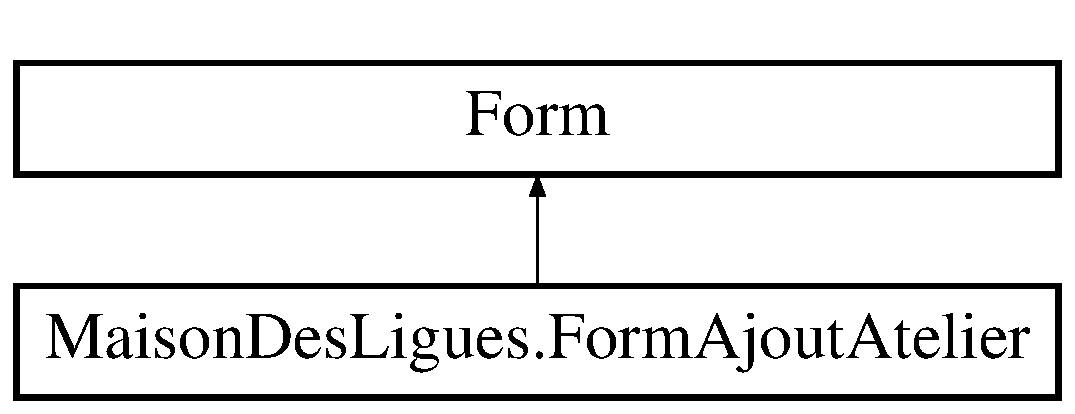
\includegraphics[height=2.000000cm]{class_maison_des_ligues_1_1_form_ajout_atelier}
\end{center}
\end{figure}
\subsection*{Protected Member Functions}
\begin{DoxyCompactItemize}
\item 
override void \hyperlink{class_maison_des_ligues_1_1_form_ajout_atelier_a52252469bf721b0bd33ba2c993944dbc}{Dispose} (bool disposing)
\begin{DoxyCompactList}\small\item\em Clean up any resources being used. \end{DoxyCompactList}\end{DoxyCompactItemize}


\subsection{Member Function Documentation}
\hypertarget{class_maison_des_ligues_1_1_form_ajout_atelier_a52252469bf721b0bd33ba2c993944dbc}{\index{Maison\+Des\+Ligues\+::\+Form\+Ajout\+Atelier@{Maison\+Des\+Ligues\+::\+Form\+Ajout\+Atelier}!Dispose@{Dispose}}
\index{Dispose@{Dispose}!Maison\+Des\+Ligues\+::\+Form\+Ajout\+Atelier@{Maison\+Des\+Ligues\+::\+Form\+Ajout\+Atelier}}
\subsubsection[{Dispose}]{\setlength{\rightskip}{0pt plus 5cm}override void Maison\+Des\+Ligues.\+Form\+Ajout\+Atelier.\+Dispose (
\begin{DoxyParamCaption}
\item[{bool}]{disposing}
\end{DoxyParamCaption}
)\hspace{0.3cm}{\ttfamily [protected]}}}\label{class_maison_des_ligues_1_1_form_ajout_atelier_a52252469bf721b0bd33ba2c993944dbc}


Clean up any resources being used. 


\begin{DoxyParams}{Parameters}
{\em disposing} & true if managed resources should be disposed; otherwise, false.\\
\hline
\end{DoxyParams}


The documentation for this class was generated from the following files\+:\begin{DoxyCompactItemize}
\item 
Maison\+Des\+Ligues/Form\+Ajout\+Atelier.\+cs\item 
Maison\+Des\+Ligues/Form\+Ajout\+Atelier.\+Designer.\+cs\end{DoxyCompactItemize}

\hypertarget{class_maison_des_ligues_1_1_form_ajout_theme}{\section{Maison\+Des\+Ligues.\+Form\+Ajout\+Theme Class Reference}
\label{class_maison_des_ligues_1_1_form_ajout_theme}\index{Maison\+Des\+Ligues.\+Form\+Ajout\+Theme@{Maison\+Des\+Ligues.\+Form\+Ajout\+Theme}}
}
Inheritance diagram for Maison\+Des\+Ligues.\+Form\+Ajout\+Theme\+:\begin{figure}[H]
\begin{center}
\leavevmode
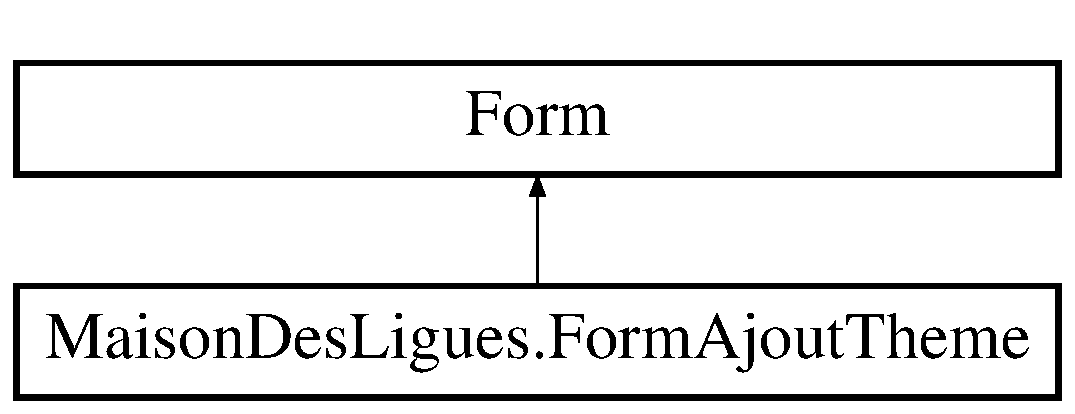
\includegraphics[height=2.000000cm]{class_maison_des_ligues_1_1_form_ajout_theme}
\end{center}
\end{figure}
\subsection*{Protected Member Functions}
\begin{DoxyCompactItemize}
\item 
override void \hyperlink{class_maison_des_ligues_1_1_form_ajout_theme_afd2a40fc9968710cba9d5e588a15980f}{Dispose} (bool disposing)
\begin{DoxyCompactList}\small\item\em Clean up any resources being used. \end{DoxyCompactList}\end{DoxyCompactItemize}


\subsection{Member Function Documentation}
\hypertarget{class_maison_des_ligues_1_1_form_ajout_theme_afd2a40fc9968710cba9d5e588a15980f}{\index{Maison\+Des\+Ligues\+::\+Form\+Ajout\+Theme@{Maison\+Des\+Ligues\+::\+Form\+Ajout\+Theme}!Dispose@{Dispose}}
\index{Dispose@{Dispose}!Maison\+Des\+Ligues\+::\+Form\+Ajout\+Theme@{Maison\+Des\+Ligues\+::\+Form\+Ajout\+Theme}}
\subsubsection[{Dispose}]{\setlength{\rightskip}{0pt plus 5cm}override void Maison\+Des\+Ligues.\+Form\+Ajout\+Theme.\+Dispose (
\begin{DoxyParamCaption}
\item[{bool}]{disposing}
\end{DoxyParamCaption}
)\hspace{0.3cm}{\ttfamily [protected]}}}\label{class_maison_des_ligues_1_1_form_ajout_theme_afd2a40fc9968710cba9d5e588a15980f}


Clean up any resources being used. 


\begin{DoxyParams}{Parameters}
{\em disposing} & true if managed resources should be disposed; otherwise, false.\\
\hline
\end{DoxyParams}


The documentation for this class was generated from the following files\+:\begin{DoxyCompactItemize}
\item 
M\+D\+L/\+Maison\+Des\+Ligues/Form\+Ajout\+Theme.\+cs\item 
M\+D\+L/\+Maison\+Des\+Ligues/Form\+Ajout\+Theme.\+Designer.\+cs\end{DoxyCompactItemize}

\hypertarget{class_maison_des_ligues_1_1_form_ajout_vacation}{\section{Maison\+Des\+Ligues.\+Form\+Ajout\+Vacation Class Reference}
\label{class_maison_des_ligues_1_1_form_ajout_vacation}\index{Maison\+Des\+Ligues.\+Form\+Ajout\+Vacation@{Maison\+Des\+Ligues.\+Form\+Ajout\+Vacation}}
}
Inheritance diagram for Maison\+Des\+Ligues.\+Form\+Ajout\+Vacation\+:\begin{figure}[H]
\begin{center}
\leavevmode
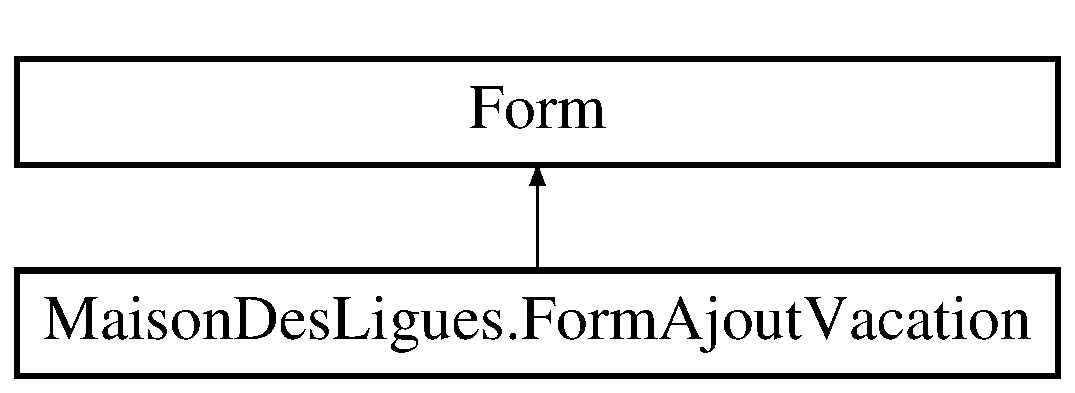
\includegraphics[height=2.000000cm]{class_maison_des_ligues_1_1_form_ajout_vacation}
\end{center}
\end{figure}
\subsection*{Protected Member Functions}
\begin{DoxyCompactItemize}
\item 
override void \hyperlink{class_maison_des_ligues_1_1_form_ajout_vacation_a15b66d7a97ec132c1cba8f7fa308e709}{Dispose} (bool disposing)
\begin{DoxyCompactList}\small\item\em Clean up any resources being used. \end{DoxyCompactList}\end{DoxyCompactItemize}


\subsection{Member Function Documentation}
\hypertarget{class_maison_des_ligues_1_1_form_ajout_vacation_a15b66d7a97ec132c1cba8f7fa308e709}{\index{Maison\+Des\+Ligues\+::\+Form\+Ajout\+Vacation@{Maison\+Des\+Ligues\+::\+Form\+Ajout\+Vacation}!Dispose@{Dispose}}
\index{Dispose@{Dispose}!Maison\+Des\+Ligues\+::\+Form\+Ajout\+Vacation@{Maison\+Des\+Ligues\+::\+Form\+Ajout\+Vacation}}
\subsubsection[{Dispose}]{\setlength{\rightskip}{0pt plus 5cm}override void Maison\+Des\+Ligues.\+Form\+Ajout\+Vacation.\+Dispose (
\begin{DoxyParamCaption}
\item[{bool}]{disposing}
\end{DoxyParamCaption}
)\hspace{0.3cm}{\ttfamily [protected]}}}\label{class_maison_des_ligues_1_1_form_ajout_vacation_a15b66d7a97ec132c1cba8f7fa308e709}


Clean up any resources being used. 


\begin{DoxyParams}{Parameters}
{\em disposing} & true if managed resources should be disposed; otherwise, false.\\
\hline
\end{DoxyParams}


The documentation for this class was generated from the following files\+:\begin{DoxyCompactItemize}
\item 
M\+D\+L/\+Maison\+Des\+Ligues/Form\+Ajout\+Vacation.\+cs\item 
M\+D\+L/\+Maison\+Des\+Ligues/Form\+Ajout\+Vacation.\+Designer.\+cs\end{DoxyCompactItemize}

\hypertarget{class_maison_des_ligues_1_1_form_modifi_vacation}{\section{Maison\+Des\+Ligues.\+Form\+Modifi\+Vacation Class Reference}
\label{class_maison_des_ligues_1_1_form_modifi_vacation}\index{Maison\+Des\+Ligues.\+Form\+Modifi\+Vacation@{Maison\+Des\+Ligues.\+Form\+Modifi\+Vacation}}
}
Inheritance diagram for Maison\+Des\+Ligues.\+Form\+Modifi\+Vacation\+:\begin{figure}[H]
\begin{center}
\leavevmode
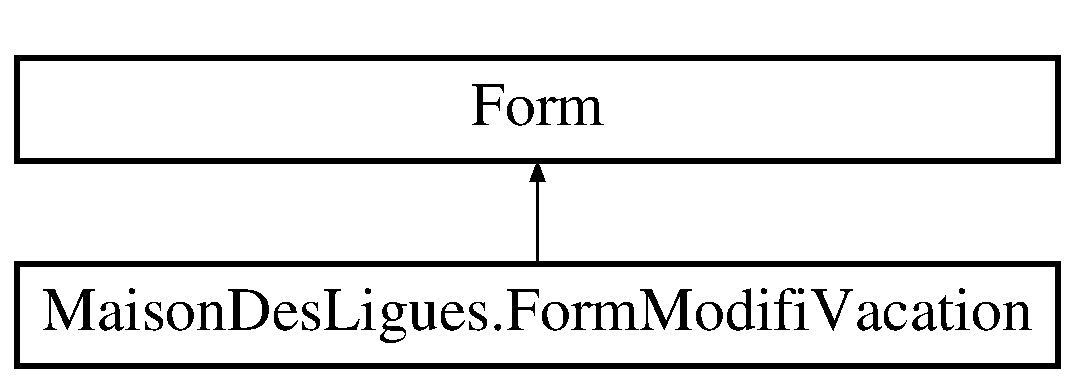
\includegraphics[height=2.000000cm]{class_maison_des_ligues_1_1_form_modifi_vacation}
\end{center}
\end{figure}
\subsection*{Protected Member Functions}
\begin{DoxyCompactItemize}
\item 
override void \hyperlink{class_maison_des_ligues_1_1_form_modifi_vacation_a585841f29765e80cf6654705ad8c20ca}{Dispose} (bool disposing)
\begin{DoxyCompactList}\small\item\em Clean up any resources being used. \end{DoxyCompactList}\end{DoxyCompactItemize}


\subsection{Member Function Documentation}
\hypertarget{class_maison_des_ligues_1_1_form_modifi_vacation_a585841f29765e80cf6654705ad8c20ca}{\index{Maison\+Des\+Ligues\+::\+Form\+Modifi\+Vacation@{Maison\+Des\+Ligues\+::\+Form\+Modifi\+Vacation}!Dispose@{Dispose}}
\index{Dispose@{Dispose}!Maison\+Des\+Ligues\+::\+Form\+Modifi\+Vacation@{Maison\+Des\+Ligues\+::\+Form\+Modifi\+Vacation}}
\subsubsection[{Dispose}]{\setlength{\rightskip}{0pt plus 5cm}override void Maison\+Des\+Ligues.\+Form\+Modifi\+Vacation.\+Dispose (
\begin{DoxyParamCaption}
\item[{bool}]{disposing}
\end{DoxyParamCaption}
)\hspace{0.3cm}{\ttfamily [protected]}}}\label{class_maison_des_ligues_1_1_form_modifi_vacation_a585841f29765e80cf6654705ad8c20ca}


Clean up any resources being used. 


\begin{DoxyParams}{Parameters}
{\em disposing} & true if managed resources should be disposed; otherwise, false.\\
\hline
\end{DoxyParams}


The documentation for this class was generated from the following files\+:\begin{DoxyCompactItemize}
\item 
M\+D\+L/\+Maison\+Des\+Ligues/Form\+Modifi\+Vacation.\+cs\item 
M\+D\+L/\+Maison\+Des\+Ligues/Form\+Modifi\+Vacation.\+Designer.\+cs\end{DoxyCompactItemize}

\hypertarget{class_maison_des_ligues_1_1_frm_login}{\section{Maison\+Des\+Ligues.\+Frm\+Login Class Reference}
\label{class_maison_des_ligues_1_1_frm_login}\index{Maison\+Des\+Ligues.\+Frm\+Login@{Maison\+Des\+Ligues.\+Frm\+Login}}
}
Inheritance diagram for Maison\+Des\+Ligues.\+Frm\+Login\+:\begin{figure}[H]
\begin{center}
\leavevmode
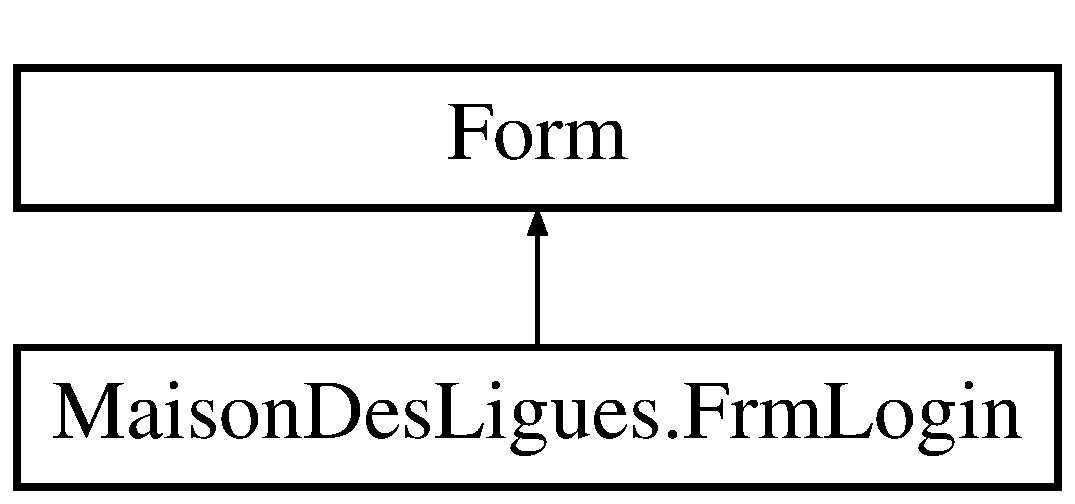
\includegraphics[height=2.000000cm]{class_maison_des_ligues_1_1_frm_login}
\end{center}
\end{figure}
\subsection*{Public Member Functions}
\begin{DoxyCompactItemize}
\item 
\hyperlink{class_maison_des_ligues_1_1_frm_login_a16d5a2efd1c29334f1a0ccf25c910b64}{Frm\+Login} ()
\begin{DoxyCompactList}\small\item\em constructeur \end{DoxyCompactList}\end{DoxyCompactItemize}
\subsection*{Protected Member Functions}
\begin{DoxyCompactItemize}
\item 
override void \hyperlink{class_maison_des_ligues_1_1_frm_login_a1b5a9829dc7217d8cca6c504b59cc9c6}{Dispose} (bool disposing)
\begin{DoxyCompactList}\small\item\em Nettoyage des ressources utilisées. \end{DoxyCompactList}\end{DoxyCompactItemize}


\subsection{Constructor \& Destructor Documentation}
\hypertarget{class_maison_des_ligues_1_1_frm_login_a16d5a2efd1c29334f1a0ccf25c910b64}{\index{Maison\+Des\+Ligues\+::\+Frm\+Login@{Maison\+Des\+Ligues\+::\+Frm\+Login}!Frm\+Login@{Frm\+Login}}
\index{Frm\+Login@{Frm\+Login}!Maison\+Des\+Ligues\+::\+Frm\+Login@{Maison\+Des\+Ligues\+::\+Frm\+Login}}
\subsubsection[{Frm\+Login}]{\setlength{\rightskip}{0pt plus 5cm}Maison\+Des\+Ligues.\+Frm\+Login.\+Frm\+Login (
\begin{DoxyParamCaption}
{}
\end{DoxyParamCaption}
)}}\label{class_maison_des_ligues_1_1_frm_login_a16d5a2efd1c29334f1a0ccf25c910b64}


constructeur 



\subsection{Member Function Documentation}
\hypertarget{class_maison_des_ligues_1_1_frm_login_a1b5a9829dc7217d8cca6c504b59cc9c6}{\index{Maison\+Des\+Ligues\+::\+Frm\+Login@{Maison\+Des\+Ligues\+::\+Frm\+Login}!Dispose@{Dispose}}
\index{Dispose@{Dispose}!Maison\+Des\+Ligues\+::\+Frm\+Login@{Maison\+Des\+Ligues\+::\+Frm\+Login}}
\subsubsection[{Dispose}]{\setlength{\rightskip}{0pt plus 5cm}override void Maison\+Des\+Ligues.\+Frm\+Login.\+Dispose (
\begin{DoxyParamCaption}
\item[{bool}]{disposing}
\end{DoxyParamCaption}
)\hspace{0.3cm}{\ttfamily [protected]}}}\label{class_maison_des_ligues_1_1_frm_login_a1b5a9829dc7217d8cca6c504b59cc9c6}


Nettoyage des ressources utilisées. 


\begin{DoxyParams}{Parameters}
{\em disposing} & true si les ressources managées doivent être supprimées ; sinon, false.\\
\hline
\end{DoxyParams}


The documentation for this class was generated from the following files\+:\begin{DoxyCompactItemize}
\item 
Maison\+Des\+Ligues/Frm\+Login.\+cs\item 
Maison\+Des\+Ligues/Frm\+Login.\+Designer.\+cs\end{DoxyCompactItemize}

\hypertarget{class_maison_des_ligues_1_1_frm_principale}{\section{Maison\+Des\+Ligues.\+Frm\+Principale Class Reference}
\label{class_maison_des_ligues_1_1_frm_principale}\index{Maison\+Des\+Ligues.\+Frm\+Principale@{Maison\+Des\+Ligues.\+Frm\+Principale}}
}
Inheritance diagram for Maison\+Des\+Ligues.\+Frm\+Principale\+:\begin{figure}[H]
\begin{center}
\leavevmode
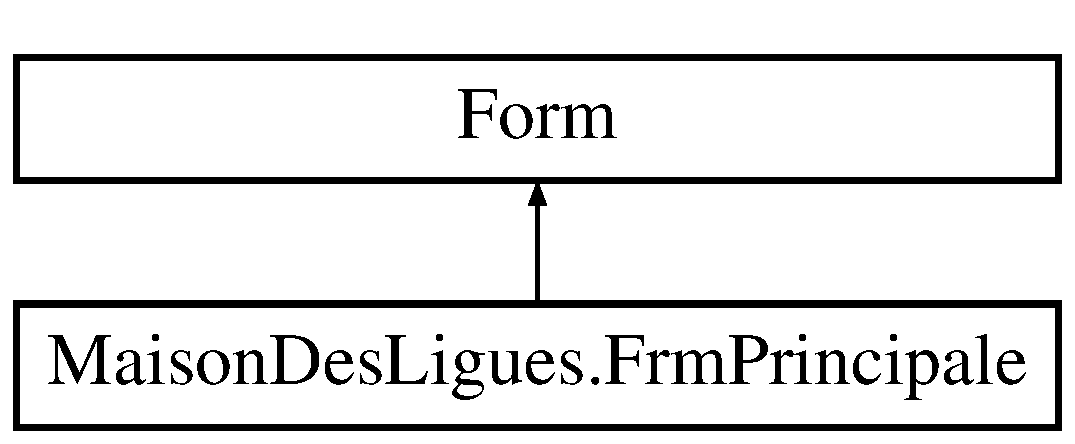
\includegraphics[height=2.000000cm]{class_maison_des_ligues_1_1_frm_principale}
\end{center}
\end{figure}
\subsection*{Public Member Functions}
\begin{DoxyCompactItemize}
\item 
\hyperlink{class_maison_des_ligues_1_1_frm_principale_a57b3b29fd74de6dba450eeddb60b0bce}{Frm\+Principale} ()
\begin{DoxyCompactList}\small\item\em constructeur du formulaire \end{DoxyCompactList}\end{DoxyCompactItemize}
\subsection*{Protected Member Functions}
\begin{DoxyCompactItemize}
\item 
override void \hyperlink{class_maison_des_ligues_1_1_frm_principale_a65be0e11ff6ef434dd448410efc60f00}{Dispose} (bool disposing)
\begin{DoxyCompactList}\small\item\em Clean up any resources being used. \end{DoxyCompactList}\end{DoxyCompactItemize}


\subsection{Constructor \& Destructor Documentation}
\hypertarget{class_maison_des_ligues_1_1_frm_principale_a57b3b29fd74de6dba450eeddb60b0bce}{\index{Maison\+Des\+Ligues\+::\+Frm\+Principale@{Maison\+Des\+Ligues\+::\+Frm\+Principale}!Frm\+Principale@{Frm\+Principale}}
\index{Frm\+Principale@{Frm\+Principale}!Maison\+Des\+Ligues\+::\+Frm\+Principale@{Maison\+Des\+Ligues\+::\+Frm\+Principale}}
\subsubsection[{Frm\+Principale}]{\setlength{\rightskip}{0pt plus 5cm}Maison\+Des\+Ligues.\+Frm\+Principale.\+Frm\+Principale (
\begin{DoxyParamCaption}
{}
\end{DoxyParamCaption}
)}}\label{class_maison_des_ligues_1_1_frm_principale_a57b3b29fd74de6dba450eeddb60b0bce}


constructeur du formulaire 



\subsection{Member Function Documentation}
\hypertarget{class_maison_des_ligues_1_1_frm_principale_a65be0e11ff6ef434dd448410efc60f00}{\index{Maison\+Des\+Ligues\+::\+Frm\+Principale@{Maison\+Des\+Ligues\+::\+Frm\+Principale}!Dispose@{Dispose}}
\index{Dispose@{Dispose}!Maison\+Des\+Ligues\+::\+Frm\+Principale@{Maison\+Des\+Ligues\+::\+Frm\+Principale}}
\subsubsection[{Dispose}]{\setlength{\rightskip}{0pt plus 5cm}override void Maison\+Des\+Ligues.\+Frm\+Principale.\+Dispose (
\begin{DoxyParamCaption}
\item[{bool}]{disposing}
\end{DoxyParamCaption}
)\hspace{0.3cm}{\ttfamily [protected]}}}\label{class_maison_des_ligues_1_1_frm_principale_a65be0e11ff6ef434dd448410efc60f00}


Clean up any resources being used. 


\begin{DoxyParams}{Parameters}
{\em disposing} & true if managed resources should be disposed; otherwise, false.\\
\hline
\end{DoxyParams}


The documentation for this class was generated from the following files\+:\begin{DoxyCompactItemize}
\item 
M\+D\+L/\+Maison\+Des\+Ligues/Frm\+Principale.\+cs\item 
M\+D\+L/\+Maison\+Des\+Ligues/Frm\+Principale.\+Designer.\+cs\end{DoxyCompactItemize}

%--- End generated contents ---

% Index
\newpage
\phantomsection
\addcontentsline{toc}{chapter}{Index}
\printindex

\end{document}
